\documentclass[../TST.tex]{subfiles}
\begin{document}
\begin{large}
	\textbf{Short Exam 1}
\end{large}

\begin{sproblem}
An axially symmetric body (e.g. a hoop, a cylinder, or a ball) of mass $m$, radius $r$, and moment of inertia $I$ has zero initial velocity and an initial angular velocity $\omega_0$. The body is placed at the base of an incline, as shown on Figure \ref{fig1}. The coefficient of friction between the body and the incline is $k$. The acceleration due to gravity is $g$.
\begin{subpart}
	\item For what values of $k$ will the body go up? \score{0.5}
	\item Assume $k$ is such that the body starts moving along the incline.\\
		What is the distance $L_1$ the body has moved until the slipping stops?	\score{1.25}\\
		What is the velocity of the body $V_1$ at that instant? \score{0.5}
	\item What additional distance $L_2$ does the body move until it stops? \score{1.0}\\
		We place three bodies at the base of the plane -- a hoop, a cylinder, and a ball (with moments of inertia $mr^2$, $\frac{1}{2}mr^2$ and $\frac{2}{5}mr^2$). The bodies are given identical initial angular velocities. Which body will rise up the most, and which the least?\score{0.25}
	\item What is the velocity $V_2$ of the body when it returns to the base of the incline? \score{1.25}\\
		Calculate $V_2$ for a hoop with $k=\sqrt{3}/2$ and $\alpha=\ang{30}$.\score{0.25}
\end{subpart}
\begin{figure}[h]
		\centering
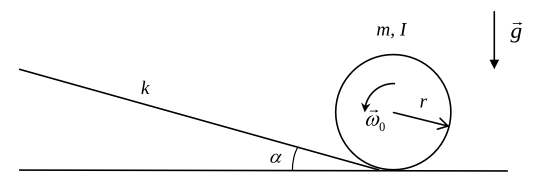
\includegraphics[width=0.7\textwidth]{fig/2010_l1.png}
    \caption{}
	\label{fig1}
\end{figure}
\end{sproblem}

\ifprob \else
\begin{solution} 
	(a) There are only three forces at play, the weight of the body $mg$, the normal force $N=mg\cos{\alpha}$ from the plane, and a frictional force $f$. We will denote the velocity of the centre of mass by $v$ and the angular velocity by $\omega$. For the body to roll without slipping, we want the velocity of the body relative to the incline  to be zero at its contact points with the incline, meaning $v-\omega r=0$. Initially $v=0$ and $\omega=\omega_0$, so the body has to slip instead. Then, if it does move, we will have sliding friction, or $f=kN=kmg\cos{\alpha}$. To move upwards, this force must overcome the component of gravity directed along the incline, $mg\sin{\alpha}$. We get $kmg\cos{\alpha}-mg\sin{\alpha}\geq 0$, or $\boxed{k\geq \tan{\alpha}.}$
\begin{center}
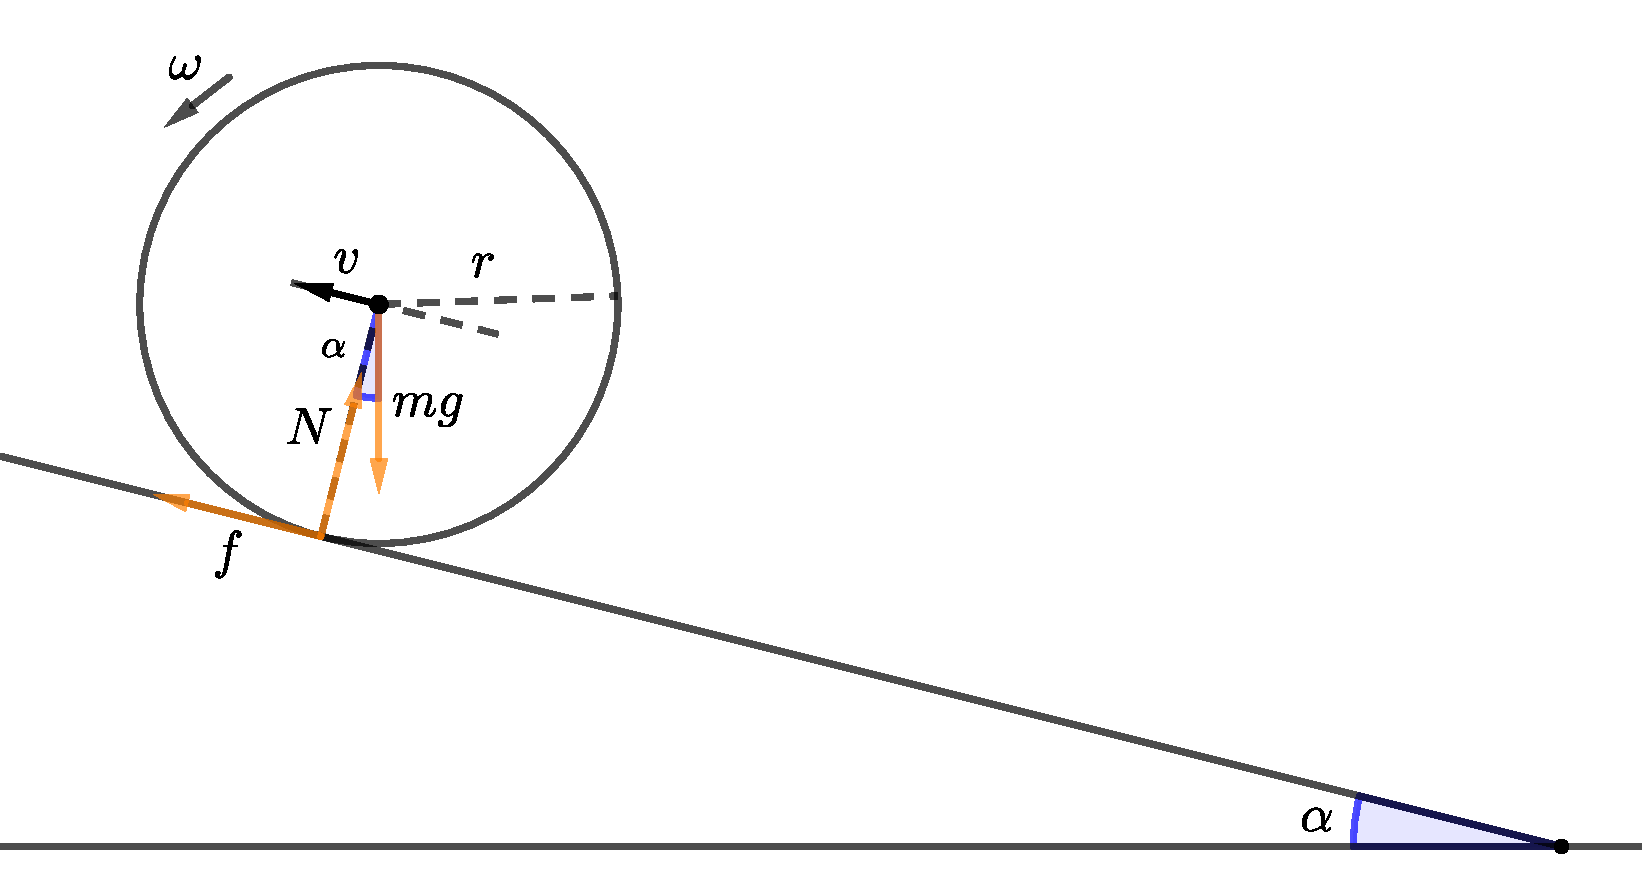
\includegraphics[width=0.6\textwidth]{fig/a2010_l1.pdf}
\end{center}
(b) The motion of the centre of mass is set by $kmg\cos{\alpha}-mg\sin{\alpha}=ma$. At $t=0$ the velocity is zero, which implies $v=(k\cos{\alpha}-\sin{\alpha})gt$. Working with positive angular velocities when the rotation is counterclockwise, the torque equation with respect to the centre of mass looks like $I \frac{\mathrm{d}\omega}{\mathrm{d}t}=-fr$. Integrating this with the initial condition $\omega(0)=\omega_0$, we find $\omega =\omega_0- \left(\frac{kmgr\cos{\alpha}}{I}\right) t$. Now, $v$ and $\omega$ will evolve this way until a time $t_1$ when $v=\omega r$. From then on, the body is locked into rolling without slipping and the friction force will change. To get $t_1$, we write
\begin{equation*}
	(k\cos{\alpha}-\sin{\alpha})gt_1=\left(\omega_0- \frac{kmgr\cos{\alpha}}{I}t_1\right)r \quad\Rightarrow\quad t_1=\frac{\omega_0r/g}{k\cos{\alpha}\left(1+\frac{mr^2}{I}\right)-\sin{\alpha}}
.
\end{equation*}
The total distance travelled is 
\begin{equation*}
L_1=\frac{at_1^2}{2}=\boxed{\frac{\omega_0^2r^2}{2g}\cdot \frac{k\cos{\alpha}-\sin{\alpha}}{\left(k\cos{\alpha}\left(1+\frac{mr^2}{I}\right)-\sin{\alpha}\right)^2}.}
\end{equation*}
The velocity at $t_1$ is
\begin{equation*}
	V_1=at_1=\boxed{\omega_0r\cdot \frac{k\cos{\alpha}-\sin{\alpha}}{k\cos{\alpha}\left(1+\frac{mr^2}{I}\right)-\sin{\alpha}}.}
\end{equation*}
(c) After the slipping stops, we always have $v=\omega r$. We differentiate this to get an additional relation, $a=\frac{\mathrm{d}\omega}{\mathrm{d}t}r$. Together  with the previous rotational and translational equations of motion, this is a system of three equations with three variables: $a$, $\frac{\mathrm{d}\omega}{\mathrm{d}t}$, and $f$. The solution is
\begin{equation*}
	a=-\frac{g\sin{\alpha}}{1+\frac{I}{mr^2}}, \quad\quad \frac{\mathrm{d}\omega}{\mathrm{d}t}=-\frac{g\sin{\alpha}}{r\left(1+\frac{I}{mr^2}\right)}, \quad\quad f=\left( \frac{mr^2}{I+mr^2}\right){mg\sin{\alpha}} .
\end{equation*}
Then, the additional distance before stopping is 
\begin{equation*}
	L_2=\frac{V_1^2}{2|a|}=\boxed{\frac{\omega_0^2r^2}{2g\sin{\alpha}}\left(1+\frac{I}{mr^2}\right)\left(\frac{k\cos{\alpha}-\sin{\alpha}}{k\cos{\alpha}\left(1+\frac{mr^2}{I}\right)-\sin{\alpha} }\right)^2  .}
\end{equation*}
The sum of $L_1$ and $L_2$ is 
\begin{equation*}
	L=\frac{\omega^2r^2}{2g}\cdot \frac{\left(k\cos{\alpha}\left(1+\frac{I}{mr^2}\right)-\frac{I}{mr^2}\sin{\alpha}\right) \left(k\cos{\alpha}-\sin{\alpha}\right)}{\left(k\cos{\alpha}\left(1+\frac{mr^2}{I}\right) -\sin{\alpha}\right)^2 \sin{\alpha}}
.
\end{equation*}
Because $k>\tan{\alpha}$, increasing $I$ would both increase the numerator and decrease the denominator of this expression. A larger $I$ means a greater distance $L$. Thus, the \fbox{hoop} rises up the \fbox{most} and the \fbox{ball} rises up the \fbox{least.}\\

(d) When the body rolls downhill, the motion is still restricted to rolling without slipping. Because there is no relative motion with respect to the incline, the friction force does zero work, and energy is conserved. We will take the base of the incline as the zero point for the potential energy. At the start of the descent, the kinetic energy is zero and the potential energy is $mgL\sin{\alpha}$. At the end, the potential energy is zero and the kinetic energy is $\frac{mV_2^2}{2}+\frac{I(V_2/r)^2}{2}$:
\begin{equation*}
	mgL\sin{\alpha}=\frac{mV_2^2}{2}\left(1+\frac{I}{mr^2}\right) 
.
\end{equation*}
We conclude that
\begin{equation*}
	\boxed{V_2=\omega_0r \left(\frac{\left(k\cos{\alpha}\left(1+\frac{I}{mr^2}\right)-\frac{I}{mr^2}\sin{\alpha}\right)\left(k\cos{\alpha}-\sin{\alpha}\right)  }{\left(1+\frac{I}{mr^2}\right)\left(k\cos{\alpha}\left(1+\frac{mr^2}{I}\right) -\sin{\alpha}\right)^2}\right)^{1/2}.}
\end{equation*}
Substituting the values for $k$ and $\alpha$, we get $\boxed{V_2=\omega_0r/\sqrt{8}.}$

\end{solution}
\fi
\ifprob 
	\clearpage
\else 
\fi
\end{document}

